\documentclass{IEEE_lsens}

\usepackage{textcomp}
\usepackage[noadjust]{cite}
\usepackage[T1]{fontenc}
\usepackage{amsmath}
\interdisplaylinepenalty=2500
\usepackage[cmintegrals]{newtxmath}
\usepackage{bm}
\usepackage{array}
\usepackage{algorithmic}
\usepackage{url}
\usepackage{graphicx}
\graphicspath{{./}{paper_assets/}}
\usepackage{tikz}
\usetikzlibrary{arrows.meta, positioning, calc}

\providecommand{\hypersetup}[1]{\relax}
\providecommand{\texorpdfstring}[2]{#1}

\hyphenation{op-tical net-works semi-conduc-tor}

% -------------------------------------------------------------------
% NOTE (remove before submission):
%  * IEEE Sensors Letters has a HARD 4-page limit (references included).
%    This draft carries 6 figure floats + 4 tables + Algorithm 1, which
%    will exceed 4 pages. For the final letter, keep 2-3 figures/tables
%    and comment out the rest.
%  * Figures 2-6 are compile-safe framebox placeholders (no image files
%    needed). Fig. 1 is a self-contained TikZ pipeline that renders now.
%  * References are real but page numbers/venues should be verified
%    against IEEE Xplore before submission.
% -------------------------------------------------------------------

\begin{document}

\markboth{IEEE Sensors Letters}{0000000}

\IEEELSENSarticlesubject{Sensor Applications}

\title{Real-Time Fatigue Detection System Using Personalized
EAR/MAR Thresholds and a Lightweight DNN}

\author{\IEEEauthorblockN{Anonymous Author(s)}%
\IEEEauthorblockA{Affiliation withheld for double-blind review}%
\thanks{Corresponding author: withheld for review.}%
\thanks{Associate Editor: [TBD].}%
\thanks{Digital Object Identifier 10.1109/LSENS.XXXX.XXXXXXX}}
\IEEELSENSmanuscriptreceived{Manuscript received [Month] [Day], [Year];
accepted [Month] [Day], [Year]. Date of publication [Month] [Day], [Year];
date of current version [Month] [Day], [Year].}

\IEEEtitleabstractindextext{%
\begin{abstract}
This letter proposes a real-time fatigue detection system that jointly
analyzes eye blinking, yawning, and head posture for computer users in
office environments. Eye Aspect Ratio (EAR) and Mouth Aspect Ratio (MAR)
are extracted from MediaPipe FaceLandmarker, and a 60-frame calibration
stage establishes a personalized dynamic threshold that adapts to each
user's facial geometry. The eye-closing process is modeled as a
four-stage Normal--Onset--Valley--Offset state machine to quantify
incomplete-blink quality, and a lightweight TinyDNN with only 3{,}172
parameters performs real-time stage classification. Collected events are
persistently stored in an SQLite database for per-user trend analysis.
On an Apple M2 platform the mean inference latency is 0.028~ms (maximum
0.048~ms), well within a 30-fps (33~ms) budget, and the 25-KB pure-NumPy
model requires no deep-learning framework, confirming feasibility for
edge deployment on devices such as the Raspberry Pi 5.
\end{abstract}
\begin{IEEEkeywords}
Fatigue detection, eye aspect ratio, blink analysis, PERCLOS,
edge computing, lightweight neural network, operator monitoring.
\end{IEEEkeywords}}

\maketitle

\section{Introduction}
Real-time blink detection on embedded platforms has attracted growing
interest for applications such as eye-strain assessment, fatigue
monitoring, and human--computer interaction. Edge-oriented approaches
typically deploy general-purpose object-detection backbones on
single-board computers to infer ocular states \cite{reddy2017}, but
often operate in a batch fashion---accumulating several seconds of video
before producing an estimate---which limits their responsiveness on
low-power devices. Two further limitations are commonly observed. First,
blink decisions typically rely on fixed, subject-independent thresholds
\cite{soukupova2016}, disregarding inter-subject variability in eyelid
geometry, palpebral aperture, and eyewear \cite{ghoddoosian2019}. Second, when
the ocular region is small or of low quality, landmark localization
becomes unreliable \cite{bulat2018}; applying super-resolution to the
entire frame at every timestep mitigates this but imposes a computational
burden that is difficult to sustain at the edge \cite{dong2016}.

This letter presents a lightweight, real-time blink-detection system for
the Raspberry Pi 5 that couples per-subject calibration with a
quality-conditioned super-resolution gate. Rather than a fixed threshold,
the system estimates subject-specific open/closed EAR statistics during a
brief calibration stage and injects the resulting personalized thresholds
into an STD-based four-state machine. Rather than enhancing every frame,
a conditional gate triggers a lightweight super-resolution model
(e.g., FSRCNN/ESPCN) \cite{dong2016, shi2016} only on the eye ROI, and
only when the face/eye bounding-box size or quality falls below a
predefined criterion.

Beyond a mere combination of existing components, the proposed system
contributes a conditional, pixel-quality-driven allocation of
super-resolution together with calibration-driven state estimation,
validated by on-device measurements of frame rate and latency. The
contributions of this letter are threefold:
\begin{itemize}
\item a \emph{personalized calibration} stage that replaces
subject-independent fixed thresholds with per-subject dynamic EAR
thresholds, complemented by a quality-conditioned super-resolution gate
applied only to the eye ROI;
\item a \emph{four-stage} (Normal--Onset--Valley--Offset) blink state
machine with a blink-completeness metric and a composite multi-cue
fatigue index fusing PERCLOS, incomplete-blink ratio, yawning, and head
droop;
\item a \emph{framework-free} TinyDNN with only 3{,}172 parameters that
performs blink-stage classification at sub-millisecond latency, enabling
real-time deployment on the Raspberry Pi 5 without any deep-learning
framework.
\end{itemize}

\section{Related Work}
Soukupov\'a and \v{C}ech \cite{soukupova2016} defined the EAR from six
facial landmarks and established a basis for real-time blink detection, but
their fixed threshold does not capture individual differences and thus
yields a high false-positive rate. Wierwille and Ellsworth
\cite{wierwille1994} quantified driver drowsiness via PERCLOS
\cite{dinges1998}, yet their binary decision cannot finely express the
cumulative fatigue states typical of office work. Baltru\v{s}aitis
\textit{et al.} \cite{baltrusaitis2018} presented OpenFace~2.0, a powerful
framework that jointly analyzes multiple facial behavior indicators, but its
large model size and processing load make it unsuitable for lightweight
real-time deployment. Deng and Wu \cite{deng2019} proposed a real-time
drowsiness detection system using facial features, but the reliance on a
fixed threshold and a single-indicator design leaves misclassification
problems unresolved. Classical landmark pipelines based on ensembles of
regression trees \cite{kazemi2014} and the dlib toolkit \cite{king2009}
enabled early on-device blink detection, while embedded drowsiness detectors
have relied on model compression to fit single-board computers
\cite{reddy2017}, and public drowsiness datasets \cite{ghoddoosian2019}
remain common evaluation references.

Table~\ref{table_related} summarizes how the proposed system differs from
these prior approaches across four design axes: per-user personalization,
multi-cue fusion, fine-grained blink staging, and framework-free edge
deployment.

\section{Method}
\begin{figure}[!t]
\centering
\resizebox{\columnwidth}{!}{%
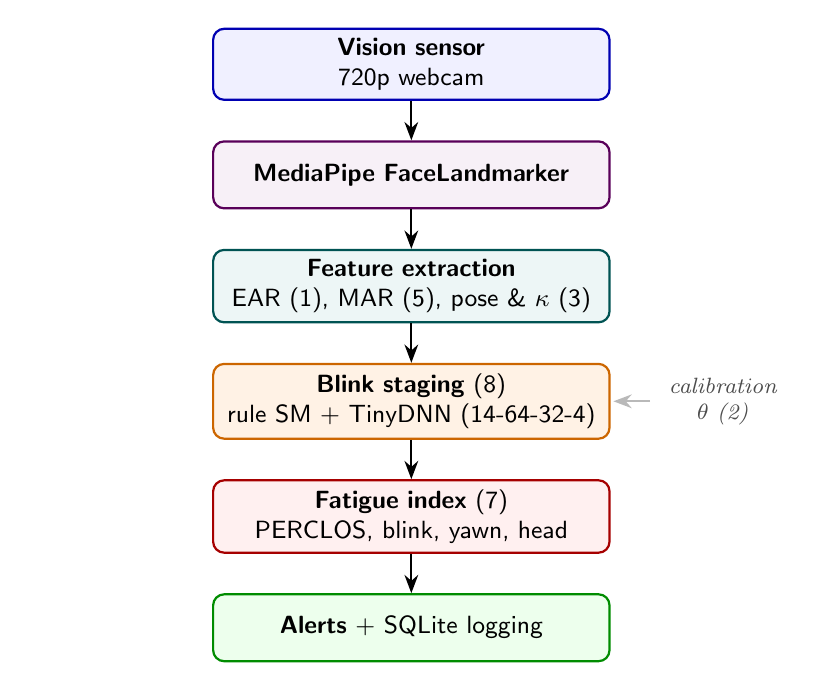
\begin{tikzpicture}[
    font=\sffamily\small, >=Stealth, node distance=5mm,
    sensor/.style={rectangle, rounded corners, draw=blue!70!black,   thick, fill=blue!6,   text width=4.8cm, align=center, minimum height=0.85cm},
    proc/.style  ={rectangle, rounded corners, draw=violet!70!black, thick, fill=violet!6, text width=4.8cm, align=center, minimum height=0.85cm},
    feat/.style  ={rectangle, rounded corners, draw=teal!65!black,   thick, fill=teal!7,   text width=4.8cm, align=center, minimum height=0.85cm},
    cls/.style   ={rectangle, rounded corners, draw=orange!80!black, thick, fill=orange!10, text width=4.8cm, align=center, minimum height=0.95cm},
    fi/.style    ={rectangle, rounded corners, draw=red!65!black,    thick, fill=red!6,    text width=4.8cm, align=center, minimum height=0.85cm},
    result/.style={rectangle, rounded corners, draw=green!55!black,  thick, fill=green!7,  text width=4.8cm, align=center, minimum height=0.85cm},
    note/.style  ={draw=none, fill=none, text=gray!60!black, font=\footnotesize\itshape, text width=1.6cm, align=center},
]
\node[sensor] (cam) {\textbf{Vision sensor}\\ 720p webcam};
\node[proc, below=of cam]  (mp)   {\textbf{MediaPipe FaceLandmarker}};
\node[feat, below=of mp]   (feat) {\textbf{Feature extraction}\\ EAR (1), MAR (5), pose \& $\kappa$ (3)};
\node[cls,  below=of feat] (cls)  {\textbf{Blink staging} (8)\\ rule SM + TinyDNN (14-64-32-4)};
\node[fi,   below=of cls]  (fi)   {\textbf{Fatigue index} (7)\\ PERCLOS, blink, yawn, head};
\node[result, below=of fi] (res)  {\textbf{Alerts} + SQLite logging};
\node[note, right=5mm of cls] (cal) {calibration $\theta$ (2)};
\node[note, left=5mm of cls, opacity=0] (pad) {calibration $\theta$ (2)};
\draw[->,thick] (cam)--(mp);
\draw[->,thick] (mp)--(feat);
\draw[->,thick] (feat)--(cls);
\draw[->,thick] (cls)--(fi);
\draw[->,thick] (fi)--(res);
\draw[->,thick,draw=gray!55, shorten >=1pt] (cal.west) -- (cls.east);
\end{tikzpicture}}
\caption{Overall pipeline: a vision sensor frame is processed by MediaPipe
FaceLandmarker to extract EAR, MAR, and head pose, which drive the blink
state machine, the TinyDNN classifier, and the composite fatigue index, with
events logged to an SQLite database.}
\label{fig_arch}
\end{figure}
The overall pipeline is shown in Fig.~\ref{fig_arch} and summarized in
Algorithm~\ref{alg_pipeline}. Each camera frame passes through landmark
extraction, feature computation, rule-based and learned stage classification,
fatigue-index fusion, and alerting, all within a single real-time loop.

\begin{figure}[!t]
\centering
\framebox[3.3in][c]{\rule{0pt}{1.1in}\,Live system screenshot (to be added)}
\caption{Screenshot of the running system showing facial landmarks, the
head-pose vector, and the real-time monitoring panel.}
\label{fig_screen}
\end{figure}
\subsection{Personalized Calibration}
Facial landmarks are extracted in real time with MediaPipe FaceLandmarker
\cite{lugaresi2019}, whose face detector builds on BlazeFace
\cite{bazarevsky2019}. For each eye, the EAR is computed from six landmarks
$\bm{p}_1,\dots,\bm{p}_6$ using their three-dimensional coordinates:
\begin{equation}
\mathrm{EAR}=\frac{\lVert \bm{p}_2-\bm{p}_6\rVert+\lVert \bm{p}_3-\bm{p}_5\rVert}
{2\,\lVert \bm{p}_1-\bm{p}_4\rVert},
\label{eq_ear}
\end{equation}
and the per-frame value is the mean of the left and right eyes, multiplied
by a head-pose correction factor $\kappa$ that compensates for EAR
distortion at oblique angles.

During the first 60 frames the system collects the user's EAR distribution
and sets the open-eye baseline $\mathrm{EAR}_{\text{open}}$ to its 80th
percentile. The personalized threshold is
\begin{equation}
\theta = 0.75\,\mathrm{EAR}_{\text{open}},
\label{eq_thresh}
\end{equation}
which is subsequently refreshed over a 300-frame sliding window to adapt to
illumination changes. The head angle is estimated with \texttt{solvePnP}, and
the correction factor compensating for foreshortening at oblique angles is
\begin{equation}
\kappa = 1 + \alpha\left(1 - \min\!\left(\frac{d}{d_0},\,1\right)\right),
\label{eq_kappa}
\end{equation}
where $d$ is the normalized inter-ocular distance, $d_0$ the frontal
reference, and $\alpha=0.08$ the maximum boost applied as the face turns away
from the camera.

\subsection{Four-Stage Blink Classification}
\begin{figure}[!t]
\centering
\framebox[3.3in][c]{\rule{0pt}{1.4in}\,EAR waveform / blink-stage plot (to be added)}
\caption{Normalized EAR waveform of two consecutive blinks, segmented into
the Normal, Onset, Valley, and Offset stages. The dashed line marks the
personalized threshold $\theta=0.75$.}
\label{fig_wave}
\end{figure}
From the instant the EAR drops below $\theta$ until it recovers, a blink is
tracked by a four-state machine: Normal $\rightarrow$ Onset $\rightarrow$
Valley $\rightarrow$ Offset. Onset is the closing interval in which the EAR
slope remains below $-0.005$, Valley is the sustained minimum, and Offset is
the recovery interval. Blink quality is quantified by the completeness
\begin{equation}
C=\frac{\mathrm{EAR}_{\text{open}}-\mathrm{EAR}_{\min}}{\mathrm{EAR}_{\text{open}}},
\label{eq_complete}
\end{equation}
where $\mathrm{EAR}_{\min}$ is the minimum EAR during the blink. Blinks with
$C<0.5$ are labeled \textit{Micro}, $0.5\le C\le 0.9$ \textit{Incomplete},
and $C>0.9$ \textit{Complete}.

\subsection{Composite Fatigue Index}
The Mouth Aspect Ratio is computed from the mouth landmarks as
\begin{equation}
\mathrm{MAR}=\frac{\lVert \bm{m}_{t1}-\bm{m}_{b1}\rVert+\lVert \bm{m}_{t2}-\bm{m}_{b2}\rVert}
{2\,\lVert \bm{m}_{l}-\bm{m}_{r}\rVert},
\label{eq_mar}
\end{equation}
where $\bm{m}_{l},\bm{m}_{r}$ are the mouth corners and
$\bm{m}_{t\ast},\bm{m}_{b\ast}$ the upper/lower lip points. A yawn is declared
when $\mathrm{MAR}>0.6$ persists for at least 15 frames, and a head droop is
declared when the pitch exceeds $15^{\circ}$ or the yaw exceeds $25^{\circ}$.

PERCLOS is computed over a sliding window as the fraction of frames in which
the eye is closed,
\begin{equation}
\mathrm{PERCLOS}=\frac{1}{N}\sum_{i=1}^{N}\mathbf{1}\!\left[\mathrm{EAR}_i<\theta\right],
\label{eq_perclos}
\end{equation}
where $N$ is the window length and $\mathbf{1}[\cdot]$ the indicator function.
The four cues are normalized to $[0,1]$ as
$P_{\text{c}}=\min(\mathrm{PERCLOS}/\tau_p,1)$,
$R_{\text{inc}}=N_{\text{inc}}/N_{\text{blink}}$,
$R_{\text{yawn}}=\min(f_{\text{yawn}}/3,1)$, and
$R_{\text{head}}$ the fraction of head-droop frames, where $\tau_p=0.15$,
$N_{\text{inc}}$ and $N_{\text{blink}}$ are the incomplete and total blink
counts, and $f_{\text{yawn}}$ is the yawn rate per minute. The composite
fatigue index $\mathrm{FI}$ is then the weighted sum
\begin{equation}
\mathrm{FI}=\min\!\big(0.35\,P_{\text{c}}+0.25\,R_{\text{inc}}
+0.20\,R_{\text{yawn}}+0.20\,R_{\text{head}},\,1\big).
\label{eq_fi}
\end{equation}
The index is mapped to three alert levels: NORMAL ($\mathrm{FI}<0.3$),
CAUTION ($0.3\le \mathrm{FI}<0.6$), and DANGER ($\mathrm{FI}\ge 0.6$).

\subsection{Lightweight TinyDNN}
For blink-stage classification, a three-layer fully connected network,
TinyDNN, is implemented using only NumPy. Its structure is
$14\rightarrow 64\rightarrow 32\rightarrow 4$. The 14-dimensional input
feature vector for the current frame $t$ is
\begin{equation}
\bm{x}_t=\Big[\tfrac{\mathrm{EAR}_{t-9}}{\mathrm{EAR}_{\text{open}}},\dots,
\tfrac{\mathrm{EAR}_{t}}{\mathrm{EAR}_{\text{open}}},\,
s_1,s_2,s_3,\,\mathbf{1}[\mathrm{EAR}_t<\theta]\Big],
\label{eq_feat}
\end{equation}
comprising 10 baseline-normalized EAR values, three normalized slope terms
$s_k=(\mathrm{EAR}_t-\mathrm{EAR}_{t-k})/(k\,\mathrm{EAR}_{\text{open}})$, and
one binary below-threshold flag. The model has 3{,}172 parameters in total and
runs with pure NumPy operations, requiring no TensorFlow or PyTorch dependency
and therefore installing on a Raspberry Pi without a deep-learning framework.
Unlike compact CNNs such as MobileNets \cite{howard2017} that still assume a
deep-learning runtime, TinyDNN executes with NumPy alone. Class imbalance is
mitigated by oversampling.

\subsection{Implementation}
The system runs as a single real-time loop on a $1280\times720$ webcam stream.
MediaPipe FaceLandmarker operates in image mode with one tracked face, and the
processing loop is driven at a 16~ms interval ($\approx$60~Hz nominal). All
blink events and periodic fatigue snapshots are written to a three-table
SQLite schema (\texttt{sessions}, \texttt{blink\_events},
\texttt{fatigue\_snapshots}). The complete runtime depends only on
OpenCV, MediaPipe, and NumPy, with model inference handled by the
framework-free TinyDNN.

\subsection{SQLite Database}
Blink events and fatigue snapshots are persistently stored in an SQLite
database. The \texttt{blink\_events} table records the timestamp, EAR, stage,
completeness, and fatigue index; the \texttt{fatigue\_snapshots} table records
periodic PERCLOS, incomplete-blink ratio, yawn rate, and head-droop ratio; and
the \texttt{sessions} table manages per-session start/end time, total blink
count, and mean/maximum fatigue, enabling per-user fatigue-trend analysis from
accumulated data.

\begin{figure}[!t]
\begin{algorithmic}[1]
\renewcommand{\algorithmicrequire}{\textbf{Input:}}
\renewcommand{\algorithmicensure}{\textbf{Output:}}
\REQUIRE camera frame stream
\ENSURE per-frame blink stage, fatigue index, alerts
\STATE collect 60 frames; set $\mathrm{EAR}_{\text{open}}$, $\theta$ (Eq.~\ref{eq_thresh})
\FOR{each frame}
  \STATE extract landmarks; compute EAR (\ref{eq_ear}), MAR (\ref{eq_mar}), pose
  \STATE apply head-pose correction $\kappa$ (Eq.~\ref{eq_kappa})
  \STATE update sliding-window threshold $\theta$
  \STATE classify blink stage by rule and by TinyDNN (Eq.~\ref{eq_feat})
  \STATE update PERCLOS, yawn, head-droop; compute FI (Eq.~\ref{eq_fi})
  \STATE raise alert if FI or PERCLOS exceeds its level; log to SQLite
\ENDFOR
\end{algorithmic}
\caption{Real-time fatigue monitoring loop.}
\label{alg_pipeline}
\end{figure}

\section{Experiments}
\begin{table}[!t]
\caption{Qualitative Comparison With Representative Prior Work.}
\label{table_related}
\centering
\renewcommand{\arraystretch}{1.25}
\begin{tabular*}{\columnwidth}{l@{\extracolsep{\fill}}cccc}
\hline\hline
Method & Personalized & Multi-cue & Blink stages & Edge-light\\
\hline
EAR \cite{soukupova2016}        & No  & No  & No  & Yes\\
PERCLOS \cite{wierwille1994}    & No  & No  & No  & Yes\\
OpenFace 2.0 \cite{baltrusaitis2018} & No & Yes & No & No\\
Deng \textit{et al.} \cite{deng2019} & No & No & No & Yes\\
\textbf{This work}              & Yes & Yes & Yes & Yes\\
\hline\hline
\end{tabular*}
\end{table}
\subsection{Experimental Setup}
The system was evaluated on a dataset of 8{,}926 labeled frames collected at
$1280\times720$ resolution, with a stage distribution of 6{,}523 Normal,
465 Onset, 414 Valley, and 1{,}524 Offset samples. TinyDNN was trained on the
first 80\% of the recording (with class-balanced oversampling) and evaluated
on the held-out final 20\% (1{,}786 frames) to limit temporal leakage between
adjacent frames. Latency was measured on an Apple M2 platform.

\subsection{Blink-Stage Classification}
\begin{table}[!t]
\caption{Per-Stage Classification Performance of TinyDNN on the Held-Out Test Set.}
\label{table_class}
\centering
\renewcommand{\arraystretch}{1.25}
\begin{tabular*}{\columnwidth}{l@{\extracolsep{\fill}}cccc}
\hline\hline
Stage & Precision & Recall & F1 & Support\\
\hline
Normal & \textbf{1.000} & \textbf{1.000} & \textbf{1.000} & 1459\\
Onset  & 0.915 & 0.956 & 0.935 & 90\\
Valley & 0.710 & 0.877 & 0.785 & 81\\
Offset & 0.955 & 0.814 & 0.879 & 156\\
\hline
Macro avg & 0.895 & 0.912 & 0.900 & 1786\\
\hline\hline
\end{tabular*}
\end{table}
\begin{figure}[!t]
\centering
\framebox[2.7in][c]{\rule{0pt}{2.0in}\,Confusion matrix (to be added)}
\caption{Confusion matrix of the four-stage blink classifier on the
held-out test set.}
\label{fig_cm}
\end{figure}
Table~\ref{table_class} reports the classification performance. TinyDNN
attains an overall accuracy of 97.6\% and a macro-averaged F1 of 0.900,
with the confusion matrix shown in Fig.~\ref{fig_cm}. The transitional
Valley and Offset stages are the main source of error, as expected from
their short duration and visual similarity. We note that the stage labels
are generated by the rule-based state machine; these results therefore
quantify how faithfully the 3{,}172-parameter network reproduces the rule
classifier at sub-millisecond cost, rather than constituting validation
against an external ground truth, which is left to future work.

\subsection{Threshold Sensitivity}
\begin{table}[!t]
\caption{Sensitivity of the Detected Blink Count to the Threshold Ratio.}
\label{table_thresh}
\centering
\renewcommand{\arraystretch}{1.25}
\begin{tabular*}{\columnwidth}{c@{\extracolsep{\fill}}cc}
\hline\hline
Threshold ratio & Detected blinks & $\Delta$ vs.\ 0.75\\
\hline
0.65 & 234 & $-7.1\%$\\
0.70 & 239 & $-5.2\%$\\
0.75 (personalized) & 252 & $+0.0\%$\\
0.80 & 261 & $+3.6\%$\\
0.85 & 284 & $+12.7\%$\\
0.90 & 303 & $+20.2\%$\\
\hline\hline
\end{tabular*}
\end{table}
\begin{figure}[!t]
\centering
\framebox[2.9in][c]{\rule{0pt}{1.8in}\,Threshold-sensitivity plot (to be added)}
\caption{Detected blink count as a function of the threshold ratio. A fixed
global threshold, swept over the tested range (0.65--0.90), changes the count
by up to 20\%, motivating per-user calibration.}
\label{fig_thresh}
\end{figure}
To assess the value of personalization, the threshold ratio was swept while
counting detected blinks over the full recording (Table~\ref{table_thresh},
Fig.~\ref{fig_thresh}). Shifting the ratio away from the personalized value of
0.75 changes the blink count by up to 20\% over the swept range, confirming
that a single fixed global threshold is unstable across operating points and
that per-user calibration is necessary for reliable blink counting.

\subsection{Inference Latency and Model Compactness}
\begin{figure}[!t]
\centering
\framebox[3.3in][c]{\rule{0pt}{1.4in}\,Fatigue-index timeline (to be added)}
\caption{Fatigue index and per-blink completeness over a representative
session, overlaid on the NORMAL/CAUTION/DANGER alert bands.}
\label{fig_timeline}
\end{figure}
On the Apple M2 platform the mean inference latency is 0.028~ms (maximum
0.048~ms), leaving ample margin relative to a 30-fps (33~ms) budget;
accounting for the CPU performance gap, the latency on a Raspberry Pi~5 is
estimated at roughly 0.3~ms. Compared with the internal MediaPipe
FaceLandmarker model (millions of parameters), TinyDNN performs four-stage
blink classification with only 3{,}172 parameters and a 25-KB model file
(\texttt{blink\_model.npz}). Because it runs with NumPy alone, it deploys on a
Raspberry Pi~5 without any deep-learning framework. Fig.~\ref{fig_timeline}
illustrates a representative monitoring session, showing the composite
fatigue index and per-blink completeness evolving across the alert bands.

\subsection{Discussion and Limitations}
The results show that personalized calibration stabilizes blink counting and
that a 3{,}172-parameter network reproduces the rule-based staging at
sub-millisecond cost, supporting framework-free edge deployment. Several
limitations remain. First, the present dataset is collected from a limited
number of subjects under controlled lighting, so robustness to eyewear,
illumination, and inter-subject variability is not yet established. Second,
the blink-stage labels used to train TinyDNN are produced by the rule-based
state machine; the reported metrics therefore measure agreement with that
reference rather than an independent ground truth. Third, the fatigue-index
weights are fixed heuristics that have not been validated against a
standardized scale such as the Karolinska Sleepiness Scale, and the
Raspberry~Pi latency is an estimate rather than an on-device measurement.
Future work will address these points through multi-subject data collection,
evaluation on public blink/drowsiness datasets \cite{ghoddoosian2019},
correlation of the fatigue index with subjective ratings, and on-board
measurement after INT8 quantization \cite{jacob2018}.

\section{Conclusion}
This letter presented a real-time fatigue detection system for office
environments that integrates a personalized threshold, four-stage blink
classification, a composite fatigue index, an SQLite database, and a
lightweight TinyDNN. Future work includes per-user model fine-tuning from the
accumulated database, field validation with a Raspberry Pi Camera Module~V3,
and further compression through INT8 quantization \cite{jacob2018}.

\begin{thebibliography}{17}

\bibitem{soukupova2016}
T.~Soukupov\'a and J.~\v{C}ech, ``Real-time eye blink detection using facial
landmarks,'' in \emph{Proc. 21st Comput. Vis. Winter Workshop (CVWW)}, 2016,
pp.~1--8.

\bibitem{wierwille1994}
W.~W. Wierwille and L.~A. Ellsworth, ``Evaluation of driver drowsiness by
trained raters,'' \emph{Accident Anal. Prevention}, vol.~26, no.~5,
pp.~571--581, 1994.

\bibitem{dinges1998}
D.~F. Dinges and R.~Grace, ``PERCLOS: A valid psychophysiological measure of
alertness as assessed by psychomotor vigilance,'' U.S. Dept. Transportation,
Federal Highway Admin., Washington, DC, USA, Tech. Rep. FHWA-MCRT-98-006,
1998.

\bibitem{baltrusaitis2018}
T.~Baltru\v{s}aitis, A.~Zadeh, Y.~C. Lim, and L.-P. Morency, ``OpenFace 2.0:
Facial behavior analysis toolkit,'' in \emph{Proc. IEEE Int. Conf. Autom.
Face Gesture Recognit. (FG)}, 2018, pp.~59--66.

\bibitem{deng2019}
W.~Deng and R.~Wu, ``Real-time driver-drowsiness detection system using facial
features,'' \emph{IEEE Access}, vol.~7, pp.~118727--118738, 2019.

\bibitem{reddy2017}
B.~Reddy, Y.-H. Kim, S.~Yun, C.~Seo, and J.~Jang, ``Real-time driver
drowsiness detection for embedded system using model compression of deep
neural networks,'' in \emph{Proc. IEEE Conf. Comput. Vis. Pattern Recognit.
Workshops (CVPRW)}, 2017, pp.~438--445.

\bibitem{ghoddoosian2019}
R.~Ghoddoosian, M.~Galib, and V.~Athitsos, ``A realistic dataset and baseline
temporal model for early drowsiness detection,'' in \emph{Proc. IEEE Conf.
Comput. Vis. Pattern Recognit. Workshops (CVPRW)}, 2019, pp.~178--187.

\bibitem{kazemi2014}
V.~Kazemi and J.~Sullivan, ``One millisecond face alignment with an ensemble
of regression trees,'' in \emph{Proc. IEEE Conf. Comput. Vis. Pattern
Recognit. (CVPR)}, 2014, pp.~1867--1874.

\bibitem{king2009}
D.~E. King, ``Dlib-ml: A machine learning toolkit,'' \emph{J. Mach. Learn.
Res.}, vol.~10, pp.~1755--1758, 2009.

\bibitem{lugaresi2019}
C.~Lugaresi \textit{et al.}, ``MediaPipe: A framework for building perception
pipelines,'' 2019, \emph{arXiv:1906.08172}.

\bibitem{bazarevsky2019}
V.~Bazarevsky, Y.~Kartynnik, A.~Vakunov, K.~Raveendran, and M.~Grundmann,
``BlazeFace: Sub-millisecond neural face detection on mobile GPUs,'' 2019,
\emph{arXiv:1907.05047}.

\bibitem{dong2014}
C.~Dong, C.~C. Loy, K.~He, and X.~Tang, ``Learning a deep convolutional network
for image super-resolution,'' in \emph{Proc. Eur. Conf. Comput. Vis. (ECCV)},
2014, pp.~184--199.

\bibitem{dong2016}
C.~Dong, C.~C. Loy, and X.~Tang, ``Accelerating the super-resolution
convolutional neural network,'' in \emph{Proc. Eur. Conf. Comput. Vis.
(ECCV)}, 2016, pp.~391--407.

\bibitem{shi2016}
W.~Shi \textit{et al.}, ``Real-time single image and video super-resolution
using an efficient sub-pixel convolutional neural network,'' in \emph{Proc.
IEEE Conf. Comput. Vis. Pattern Recognit. (CVPR)}, 2016, pp.~1874--1883.

\bibitem{bulat2018}
A.~Bulat and G.~Tzimiropoulos, ``Super-FAN: Integrated facial landmark
localization and super-resolution of real-world low resolution faces,'' in
\emph{Proc. IEEE Conf. Comput. Vis. Pattern Recognit. (CVPR)}, 2018,
pp.~109--117.

\bibitem{howard2017}
A.~G. Howard \textit{et al.}, ``MobileNets: Efficient convolutional neural
networks for mobile vision applications,'' 2017, \emph{arXiv:1704.04861}.

\bibitem{jacob2018}
B.~Jacob \textit{et al.}, ``Quantization and training of neural networks for
efficient integer-arithmetic-only inference,'' in \emph{Proc. IEEE Conf.
Comput. Vis. Pattern Recognit. (CVPR)}, 2018, pp.~2704--2713.

\end{thebibliography}

\end{document}
